\documentclass[journal,12pt,onecolumn]{IEEEtran}
\usepackage{cite}
\usepackage{graphicx}
\usepackage{amsmath,amssymb,amsfonts,amsthm}
\usepackage{algorithmic}
\usepackage{graphicx}
\usepackage{textcomp}
\usepackage{xcolor}
\usepackage{txfonts}
\usepackage{listings}
\usepackage{enumitem}
\usepackage{tfrupee}
\usepackage{listings}
\usepackage{pgf-pie}
\usepackage{mathtools,tfrupee}
\usepackage{gensymb}
\usepackage{comment}
\usepackage[breaklinks=true]{hyperref}
\usepackage{tkz-euclide} 
\usepackage{listings}
\usepackage{gvv}                                        
%\def\inputGnumericTable{}                                 
\usepackage[latin1]{inputenc} 
\usetikzlibrary{arrows.meta, positioning}
\usepackage{xparse}
\usepackage{color}                                            
\usepackage{array}                                            
\usepackage{longtable}                                       
\usepackage{calc}                                             
\usepackage{multirow}
\usepackage{multicol}
\usepackage{caption}
\usepackage{hhline}                                           
\usepackage{ifthen}                                           
\usepackage{lscape}
\usepackage{tabularx}
\usepackage{array}
\usepackage{float}
\newtheorem{theorem}{Theorem}[section]
\newtheorem{problem}{Problem}
\newtheorem{proposition}{Proposition}[section]
\newtheorem{lemma}{Lemma}[section]
\newtheorem{corollary}[theorem]{Corollary}
\newtheorem{example}{Example}[section]
\newtheorem{definition}[problem]{Definition}
\newcommand{\BEQA}{\begin{eqnarray}}
\newcommand{\EEQA}{\end{eqnarray}}
\usepackage{float}
%\newcommand{\define}{\stackrel{\triangle}{=}}
\theoremstyle{remark}
\usepackage{circuitikz}
\usepackage{tikz}
\usepackage{wrapfig}
\graphicspath{{figs/}}                                                                       
\title{Production and Industrial Engineering}

\author{EE25BTECH11023-Venkata Sai}
\begin{document}

\maketitle
\textbf{General Aptitude}

\begin{enumerate}
    \item Courage : Bravery :: Yearning : \dots

Select the most appropriate option to complete the analogy.
\begin{enumerate}
\begin{multicols}{2}
\item Longing
\item Yelling
\item Yawning
\item Glaring
\end{multicols}
\end{enumerate}
\hfill (GATE PI 2025)

\item We \dots tennis in the lawn when it suddenly started to rain.

Select the most appropriate option to complete the above sentence.

\begin{enumerate}
\item have been playing
\item had been playing
\item would have been playing
\item could be playing
\end{enumerate}

\hfill (GATE PI 2025)

\item A $4\times4$ digital image has pixel intensities $\brak{U}$ as shown in the figure. The number of pixels with $U\le 4$ is:

\begin{tabular}[12pt]{ |c| c| c| c| }
\hline
$\beta$ & Airplane A & Airplane B & Airplane C \\
\hline
$\beta = -5\,\mathrm{deg}$ & $-0.030$ & $-0.025$ & $0.040$\\
\hline
$\beta = 0\,\mathrm{deg}$ & $0$ & $0$ & $0$ \\
\hline
$\beta = 5\,\mathrm{deg}$ & $0.030$ & $0.025$ & $-0.040$\\
\hline
\end{tabular}


\begin{enumerate}
\item 3
\item 8
\item 11
\item 9
\end{enumerate}

\hfill (GATE PI 2025)

\item In the given figure, the numbers associated with the rectangle, triangle, and ellipse are 1, 2, and 3, respectively. Which one among the given options is the most appropriate combination of P, Q, and R?

 \begin{figure}[H]
\centering
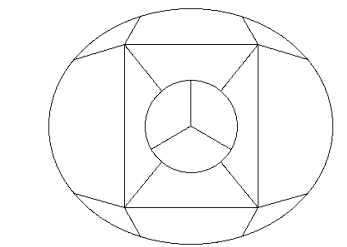
\includegraphics[width=0.5\columnwidth]{fig1.png}
\caption{}
\end{figure}

\begin{enumerate}
\begin{multicols}{2}
\item P = 6; Q = 5; R = 3
\item P = 5; Q = 6; R = 3
\item P = 3; Q = 6; R = 6
\item P = 5; Q = 3; R = 6
\end{multicols}
\end{enumerate}

\hfill (GATE PI 2025)

\item A rectangle has a length $L$ and a width $W$, where $L>W$. If the width, $W$, is increased by $10\%$, which one of the following statements is correct for all values of $L$ and $W$?

\begin{enumerate}
\item Perimeter increases by $10\%$.
\item Length of the diagonals increases by $10\%$.
\item Area increases by $10\%$.
\item The rectangle becomes a square.
\end{enumerate}

\hfill (GATE PI 2025)

\item Column-I has statements made by Shanthala; and, Column-II has responses given by Kanishk.

\begin{table}[h!]
\small
\setlength{\tabcolsep}{4pt}
\renewcommand{\arraystretch}{0.9}
\centering
\begin{tabular}{|c|c|c|p{1.8cm}|p{2.5cm}|c|}
\hline
Q. No & Type & Section & Key & Marks \\
\hline
1  & MCQ & GA & C         & 1 \\
\hline
2  & MCQ & GA & A         & 1 \\
\hline
3  & MCQ & GA & A         & 1 \\
\hline
4  & MCQ & GA & A         & 1 \\
\hline
5  & MCQ & GA & D         & 1 \\
\hline
6  & MCQ & GA & D         & \textbf{2} \\
\hline
7  & MCQ & GA & B         & 2 \\
\hline
8  & MCQ & GA & C         & 2 \\
\hline
9  & MCQ & GA & B         & 2 \\
\hline
10 & MCQ & GA & C         & 2 \\
\hline
11 & MCQ & EY & D         & 1 \\
\hline
12 & MCQ & EY & D         & 1 \\
\hline
13 & MCQ & EY & A; D      & 1 \\
\hline
14 & MCQ & EY & B         & 1 \\
\hline
15 & NAT & EY & 7.99 : 8.10 & 1 \\
\hline
16 & MCQ & EY & B         & 1 \\
\hline
17 & MCQ & EY & C         & 1 \\
\hline
18 & MCQ & EY & D         & 1 \\
\hline
19 & NAT & EY & 9.9 : 10.1  & 1 \\
\hline
20 & MCQ & EY & C         & 1 \\
\hline
21 & MCQ & EY & B         & 1 \\
\hline
22 & MCQ & EY & A         & 1 \\
\hline
23 & MCQ & EY & D         & 1 \\
\hline
24 & MCQ & EY & B         & 1 \\
\hline
25 & MCQ & EY & A         & 1 \\
\hline
26 & MCQ & EY & C         & 2 \\
\hline
27 & MCQ & EY & D         & 2 \\
\hline
28 & MCQ & EY & C         & 2 \\
\hline
29 & MCQ & EY & D         & 2 \\
\hline
30 & MCQ & EY & B         & 2 \\
\hline
31 & MCQ & EY & A         & 2 \\
\hline
32 & MCQ & EY & C         & 2 \\
\hline
33 & MCQ & EY & A         & 2 \\
\hline
34 & MCQ & EY & B         & 2 \\
\hline
35 & MCQ & EY & A         & 2 \\
\hline
36 & MCQ & EY & A         & 2 \\
\hline
37 & MCQ & EY & C         & 2 \\
\hline
38 & MCQ & EY & A         & 2 \\
\hline
39 & NAT & EY & 0.17 : 0.19 & 2 \\
\hline
40 & MCQ & EY & A         & 2 \\
\hline
41 & MCQ & EY & B         & 2 \\
\hline
42 & MCQ & EY & B         & 2 \\
\hline
43 & MCQ & EY & A         & 2 \\
\hline
44 & MCQ & EY & D         & 2 \\
\hline
45 & MCQ & EY & B         & 2 \\
\hline
46 & MCQ & EY & A         & 2 \\
\hline
47 & NAT & EY & 0.175 : 0.20 & 2 \\
\hline
48 & MCQ & EY & A         & 2 \\
\hline
49 & NAT & EY & 0.49 : 0.51  & 2 \\
\hline
50 & MCQ & EY & B         & 2 \\
\hline
51 & MCQ & EY & A         & 2 \\
\hline
52 & MCQ & EY & C         & 2 \\
\hline
53 & NAT & EY & 1660 : 1700 & 2 \\
\hline
54 & NAT & EY & 0.45 : 0.55 & 2 \\
\hline
55 & MCQ & EY & A         & 2 \\
\hline
\end{tabular}
\caption{GATE 2016 EY Answer Key Summary}
\end{table}

Identify the option that has the correct match between Column-I and Column-II.

\begin{enumerate}
\item P - 2; Q - 3; R - 1; S - 4
\item P - 3; Q - 4; R - 1; S - 2
\item P - 4; Q - 1; R - 2; S - 3
\item P - 1; Q - 2; R - 4; S - 3
\end{enumerate}

\hfill (GATE PI 2025)

\item Weight of a person can be expressed as a function of their age. The function usually varies from person to person. Suppose this function is identical for two brothers, and it monotonically increases till the age of 50 years and then it monotonically decreases. Let $a_1$ and $a_2$ (in years) denote the ages of the brothers and $a_1<a_2$.

Which one of the following statements is correct about their age on the day when they attain the same weight?

\begin{enumerate}
\begin{multicols}{2}
\item $a_1<a_2<50$
\item $a_1<50<a_2$
\item $50<a_1<a_2$
\item Either $a_1=50$ or $a_2=50$
\end{multicols}
\end{enumerate}

\hfill (GATE PI 2025)

\item A regular dodecagon (12-sided regular polygon) is inscribed in a circle of radius r cm as shown in the figure. The side of the dodecagon is d cm. All the triangles (numbered $1$ to $12$) in the figure are used to form squares of side r cm and each numbered triangle is used only once to form a square.

The number of squares that can be formed and the number of triangles required to form each square, respectively, are:
\begin{figure}[H]
\centering
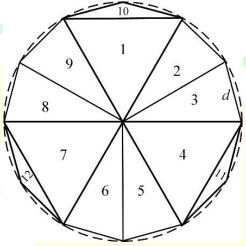
\includegraphics[width=0.3\columnwidth]{fig2.png}
\caption{}
\end{figure}

\begin{enumerate}
\begin{multicols}{4}
\item $3;4$
\item $4;3$
\item $3;3$
\item $3;2$
\end{multicols}
\end{enumerate}

\hfill (GATE PI 2025)

\item If a real variable x satisfies $3^{x^2}=27\times 9^{x}$, then the value of $\frac{2^{x^2}}{(2^{x})^{2}}$ is:

\begin{enumerate}
\begin{multicols}{4}
\item $2^{-1}$
\item $2^{0}$
\item $2^{3}$
\item $2^{15}$
\end{multicols}
\end{enumerate}

\hfill (GATE PI 2025)

\item The number of patients per shift \brak{X} consulting Dr. Gita in her past 100 shifts is shown in the figure. If the amount she earns is $\rupee 1000\brak{X-0.2}$, what is the average amount (in $\rupee$) she has earned per shift in the past $100$ shifts?

Note: The figure shown is representative.

\begin{figure}[H]
\centering
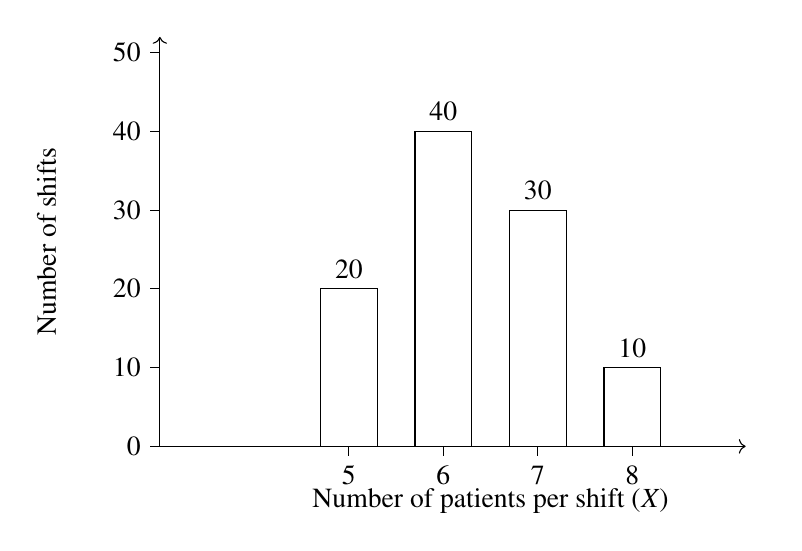
\begin{tikzpicture}[x=1.2cm,y=0.1cm]

\draw[->] (3,0) -- (9.2,0) node[below] {};
\draw[->] (3,0) -- (3,52) node[left] {};
\node at (6.5,-7) {Number of patients per shift $(X)$ };
\node[rotate=90] at (1.8,26) {Number of shifts};

\foreach \x/\lbl in {5/5,6/6,7/7,8/8}{
  \draw (\x,0) -- (\x,-1.2) node[below] {\lbl};
}

\foreach \y in {0,10,20,30,40,50}{
  \draw (3,\y) -- (2.9,\y) node[left] {\y};
}

\draw[fill=white] (4.7,0) rectangle (5.3,20);
\draw[fill=white] (5.7,0) rectangle (6.3,40);
\draw[fill=white] (6.7,0) rectangle (7.3,30);
\draw[fill=white] (7.7,0) rectangle (8.3,10);


\node at (5,22.5) {20};
\node at (6,42.5) {40};
\node at (7,32.5) {30};
\node at (8,12.5) {10};

\node at (9.4,0) {};


\end{tikzpicture}
\caption{}
\end{figure}

\begin{enumerate}
\begin{multicols}{4}
\item 6,100
\item 6,300
\item 6,000
\item 6,500
\end{multicols}
\end{enumerate}

\hfill (GATE PI 2025)

\item The eigenvalues of the matrix 
$
\myvec{
0 &  -1\\
1 & 0 
}
$ are

\begin{enumerate}
\begin{multicols}{2}
\item $-\sqrt{-1}$ and $\sqrt{-1}$
\item -1 and 1
\item $1+\sqrt{-1}$ and $1-\sqrt{-1}$
\item $-1+\sqrt{-1}$ and $-1-\sqrt{-1}$
\end{multicols}
\end{enumerate}

\hfill (GATE PI 2025)

\item If $\mathbf{i}$, $\mathbf{j}$ and $\mathbf{k}$ are the orthogonal unit vectors in Cartesian $x$-$y$-$z$ coordinate system, the curl of the vector $-2y\,\mathbf{i}+x\,\mathbf{j}$ is

\begin{enumerate}
\begin{multicols}{4}
\item $3\mathbf{k}$
\item $-3\mathbf{k}$
\item $-\mathbf{k}$
\item $\mathbf{k}$
\end{multicols}
\end{enumerate}

\hfill (GATE PI 2025)

\item If $F\brak{s}$ denotes the Laplace transform of some function $f\brak{t}$, then the Laplace transform of $e^{bt}f\brak{t}$, where b is a real constant, is

\begin{enumerate}
\begin{multicols}{2}
\item $F\brak{s-b}$
\item $F\brak{s+b}$
\item $-F\brak{s}$
\end{multicols}
\end{enumerate}

\hfill (GATE PI 2025)

\item Which one of the following equations is a linear differential equation?

\begin{enumerate}
\begin{multicols}{2}
\item $\frac{dy}{dx}+2x=y^{2}$
\item $x^{3}\frac{dy}{dx}+xy=x^{2}$
\item $x^{2}\frac{d^{2}y}{dx^{2}}+2y\frac{dy}{dx}=0$
\item $\left(\frac{dy}{dx}\right)^{2}+2x=y$
\end{multicols}
\end{enumerate}

\hfill (GATE PI 2025)

\item A bag contains $5$ red, $7$ green and $3$ blue balls. Two balls are drawn at random from the bag one-by-one. The probability of the second drawn ball being red is

\begin{enumerate}
\begin{multicols}{4}
\item $\frac{1}{5}$
\item $\frac{1}{3}$
\item $\frac{2}{5}$
\item $\frac{2}{3}$
\end{multicols}
\end{enumerate}

\hfill (GATE PI 2025)

\item Exit-hole occurrence is common in

\begin{enumerate}
\begin{multicols}{2}
\item Electron Beam Welding
\item Submerged Arc Welding
\item Friction Welding
\item Friction Stir Welding
\end{multicols}
\end{enumerate}

\hfill (GATE PI 2025)

\item An aircraft has two engines, each having a reliability $R$. The aircraft will crash only when both engines stop working. The reliability of the aircraft flying without crash is

\begin{enumerate}
\begin{multicols}{2}
\item $R^{2}$
\item $2R$
\item $2R-R^{2}$
\item $R^{2}-2R$
\end{multicols}
\end{enumerate}

\hfill (GATE PI 2025)

\item The proper sequence of design of a product is

\begin{enumerate}
\item Conceptual design, Embodiment design, Detailed design
\item Conceptual design, Detailed design, Embodiment design
\item Embodiment design, Conceptual design, Detailed design
\item Embodiment design, Detailed design, Conceptual design
\end{enumerate}

\hfill (GATE PI 2025)

\item In a work sampling, out of $n$ observations, a worker was sitting idle in $x$ observations. The standard deviation of the mean proportion of idle time is given by

\begin{enumerate}
\begin{multicols}{2}
\item $\sqrt{\frac{x^{2}}{n^{3}}}$
\item $\sqrt{\frac{x(n-x)}{n^{3}}}$
\item $\sqrt{\frac{x(n-x)}{n^{2}}}$
\item $\frac{x}{n}$
\end{multicols}
\end{enumerate}

\hfill (GATE PI 2025)

\item Atomic packing factor of a body centered cubic structure is closest to

\begin{enumerate}
\begin{multicols}{4}
\item 0.34
\item 0.52
\item 0.68
\item 0.74
\end{multicols}
\end{enumerate}

\hfill (GATE PI 2025)

\item Which one of the following statements is FALSE with respect to the injection molding of polymer composite?

\begin{enumerate}
\item Molten polymer along with the reinforcements is injected into a closed mold cavity.
\item Material deforms plastically to adopt the shape of the mold cavity.
\item Melt temperature, injection speed and screw speed are some important process parameters.
\item Commonly used reinforcements are particles, whiskers and short fibers.
\end{enumerate}

\hfill (GATE PI 2025)

\item A through hole of $8$ mm diameter is to be drilled in a $30$ mm thick mild steel plate. Which one of the following processes is the most appropriate to achieve high dimensional accuracy with less processing time?

\begin{enumerate}
\item Conventional drilling using a carbide drill bit
\item Die sinking EDM using a copper electrode
\item ECM using a copper electrode
\item Plasma arc machining
\end{enumerate}

\hfill (GATE PI 2025)

\item Which one of the following casting defects is caused due to the supply of the molten metal through two gates?
\begin{enumerate}
\begin{multicols}{2}
\item Cold shut
\item Shift
\item Pin hole
\item Rat tail
\end{multicols}
\end{enumerate}

\hfill (GATE PI 2025)

\item Match the following with reference to the CNC machine and its minimum number of axes available in the machine.

\begin{center}
\begin{tabular}{|p{1cm}|p{3cm}|p{1cm}|p{7cm}|}
\hline

\multicolumn{2}{|c|}{Process} & \multicolumn{2}{c|}{Application} \\
\hline
P & Extrusion & 1 & Producing complex parts with close tolerance \\
\hline
Q & Injection molding & 2 & Producing thermosetting plastic components \\
\hline
R & Blow molding & 3 & Producing long uniform sections \\
\hline
S & Compression molding & 4 & Producing hollow shapes \\
\hline
\end{tabular}
\end{center}

\begin{enumerate}
\begin{multicols}{2}
\item P - i, Q - ii
\item P - ii, Q - i
\item P - i, Q - iii
\item P - ii, Q - iii
\end{multicols}
\end{enumerate}

\hfill (GATE PI 2025)

\item A simply supported beam $AB$ of span $L$ is shown in the figure. A moment $M$ is applied at point $C$. The magnitude of the reaction force at point $A$ is

\begin{figure}[H]
\centering
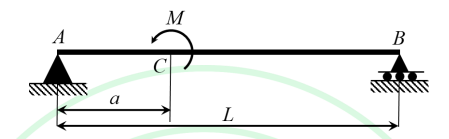
\includegraphics[width=0.5\columnwidth]{fig4.png}
\caption{}
\end{figure}

\begin{enumerate}
\begin{multicols}{4}
\item $\frac{M}{L}$
\item $\frac{M}{a}$ 
\item $\frac{M}{\,L-a\,}$
\item $\frac{M}{\,L+a\,}$
\end{multicols}
\end{enumerate}

\hfill (GATE PI 2025)

\item The relationship between the hoop stress $\sigma_{1}$ and the longitudinal stress $\sigma_{2}$ of a closed cylindrical thin-walled pressure vessel is

\begin{enumerate}
\begin{multicols}{2}
\item $\sigma_{1}=2\sigma_{2}$
\item $\sigma_{1}=\sigma_{2}$
\item $\sigma_{1}=\frac{\sigma_{2}}{2}$
\item $\sigma_{1}=\frac{1}{3}\sigma_{2}$
\end{multicols}
\end{enumerate}

\hfill (GATE PI 2025)

\item The starting simplex table of a linear programming problem is given below, where $S_1$, $S_2$, $S_3$ and $S_4$ are the slack variables. The objective of the problem is
\begin{align*}
\text{Maximize } z=6x_1+4x_2
\end{align*}
The leaving variable among the basic variables is

\begin{tabular}[12pt]{ |c| c| c| c| c| c| }
    \hline
   Q.No. & Session & Que.Type & Sec. Name & Key & Marks \\
    \hline
    46 & 4 & NAT & AE & 149.0 to 151.0 & 2\\
    \hline
    47 & 4 & NAT & AE & 1712.0 to 1719.0 & 2\\
    \hline
    48 & 4 & NAT & AE & 91 to 93 & 2\\
    \hline
    49 & 4 & NAT & AE & 87 to 89 & 2\\
    \hline
    50 & 4 & NAT & AE & 27.0 to 27.2 & 2\\
    \hline
    51 & 4 & NAT & AE & 1.43 to 1.45 & 2\\
    \hline
    52 & 4 & NAT & AE & 0.61 to 0.63 & 2\\
    \hline
    53 & 4 & NAT & AE & 3.74 to 3.76 & 2\\
    \hline
    54 & 4 & NAT & AE & 62.95 to 63.08 & 2\\
    \hline
    55 & 4 & NAT & AE & 57.10 to 60.00 & 2\\
    \hline
\end{tabular}


\begin{enumerate}
\begin{multicols}{4}
\item $S_1$
\item $S_2$
\item $S_3$
\item $S_4$
\end{multicols}
\end{enumerate}

\hfill (GATE PI 2025)

\item For an ideal Diesel cycle, the heat addition is an

\begin{enumerate}
\begin{multicols}{2}
\item isobaric process
\item isothermal process
\item isochoric process
\item isentropic process
\end{multicols}
\end{enumerate}

\hfill (GATE PI 2025)

\item Three principal stresses at a point in a material are 300 MPa, 250 MPa and 100 MPa. If the yielding just starts at that point, the yield strength (in MPa) of the material as per Tresca criterion is \dots. (Answer in integer)

\hfill (GATE PI 2025)

\item In an orthogonal straight turning process, the feed is 0.1 mm/rev and the depth of cut is $0.5$ mm. In ASA system, the side cutting edge angle of the cutting tool is $0^\circ$. The width (in mm) of the chip is \dots. (Rounded off to one decimal place)

\hfill (GATE PI 2025)

\item The pitch of the single-start lead screw of a lathe is 6 mm. It is used to cut double start thread of 3 mm pitch on a cylindrical work piece. During the thread cutting, the spindle rotates at 400 revolutions per minute (RPM). The speed (in RPM) of the lead screw is \dots. (Answer in integer)

\hfill (GATE PI 2025)

\item Two options are available to meet the annual demand of batteries in a toy company. In option 1, batteries are manufactured in the plant having fixed cost of Rupees 2,00,000 and a variable cost of Rupees 70 per unit. Option 2 consists of buying batteries from the market at a price of Rupees 90 per unit. The annual demand (in number of batteries) at which the company should switch from buying to making the batteries in the plant is \dots. (Answer in integer)

\hfill (GATE PI 2025)

\item A company estimates the demand of 2000 bulbs for the next year. The ordering cost is Rupees 300 per order and the annual carrying cost per bulb is Rupees 30. The economic order quantity (number of bulbs) is \dots. (Answer in integer)

\hfill (GATE PI 2025)

\item While inspecting final assembly of automobile-gear-boxes, 15 features were considered critical-to-quality (CTQ). During last quarter, 40000 gear boxes were produced among which 1500 defects were found of the CTQ features. The defects per million opportunities (DPMO) is \dots. (Answer in integer)

\hfill (GATE PI 2025)

\item The hole and the shaft dimensions (in mm) are given as
\begin{align*}
\text{Hole dimension}=30^{+0.04}_{-0.02} \\
\text{Shaft dimension}=30^{+0.06}_{-0.03}
\end{align*}

The maximum possible clearance (in mm) is \dots. (Rounded off to two decimal places)

\hfill (GATE PI 2025)

\item The solution of the linear differential equation
\begin{align*}
\frac{dy}{dx}+y=e^{x},
\end{align*}
when $y\brak{0}=0$, is

\begin{enumerate}
\begin{multicols}{2}
\item $y=\frac{1}{2}e^{x}-\frac{1}{2}e^{-x}$
\item $y=\frac{1}{2}e^{x}+\frac{1}{2}e^{-x}$
\item $y=e^{x}-e^{-x}$
\item $y=e^{x}+e^{-x}$
\end{multicols}
\end{enumerate}

\hfill (GATE PI 2025)

\item Which one of the following functions is analytic, given $i=\sqrt{-1}$?

\begin{enumerate}
\item $e^{x} \brak{\cos y+i\sin y }$
\item $e^{x} \brak{\cos y-i\sin y }$
\item $e^{x} \brak{-\cos y+i\sin y}$
\item $e^{-x} \brak{\cos y+i\sin y }$
\end{enumerate}

\hfill (GATE PI 2025)

\item Match the following with reference to the machining process and its feature.

\begin{table}[H]
\centering
\begin{tabular}{|c|c|c|c|}
\hline
\textbf{Activity} & \textbf{Optimistic time (days)} & \textbf{Most likely time (days)} & \textbf{Pessimistic time (days)} \\
\hline
1-2 & 1 & 2 & 3 \\
1-3 & 5 & 6 & 7 \\
1-4 & 3 & 5 & 7 \\
2-5 & 5 & 7 & 9 \\
3-5 & 2 & 4 & 6 \\
5-6 & 4 & 5 & 6 \\
4-7 & 4 & 6 & 8 \\
6-7 & 2 & 3 & 4 \\
\hline
\end{tabular}
\caption{Activity Time Estimates}
\end{table}


\begin{enumerate}
\item P - 3, Q - 4, R - 1, S - 2
\item P - 4, Q - 3, R - 2, S - 1
\item P - 4, Q - 2, R - 1, S - 3
\item P - 1, Q - 2, R - 3, S - 4
\end{enumerate}

\hfill (GATE PI 2025)

\item Match the operation/phenomenon in a grinding process with the corresponding definition listed in the table.


\begin{center}
\begin{tabular}{|c|c|c|}
\hline
\textbf{Activity} & \textbf{Activity time (in days)} & \textbf{Immediate predecessor(s)} \\
\hline
A & 2 & - \\
B & 3 & - \\
C & 2 & A \\
D & 4 & A, B \\
E & 4 & C \\
F & 3 & C \\
G & X & D, E \\
H & 2 & F, G \\
\hline
\end{tabular}
\end{center}

\begin{enumerate}
\item P - 4, Q - 1, R - 3, S - 2
\item P - 2, Q - 3, R - 1, S - 4
\item P - 2, Q - 4, R - 1, S - 3
\item P - 4, Q - 3, R - 1, S - 2
\end{enumerate}

\hfill (GATE PI 2025)

\item A CNC vertical milling is used for cutting a straight line slot in $x$-$y$ plane. Cutter is located at point $P$. The slope $\brak{\frac{dy}{dx}}$ of the straight line created by the cutter is $1.25$. Feed rate of $x$-axis is $120$ mm/min. The new position of the cutter after $20$ seconds is

\begin{figure}[H]
\centering
\begin{tikzpicture}[scale=0.9]

\draw[->] (0,0) -- (0,3.5) node[above] {$y$};
\draw[->] (0,0) -- (5.5,0) node[right] {$x$};

\fill (1,0.5) circle (2pt);
\node[right] at (1,0.5) {$P\,(10,\,5)$};

\node at (2.8,-0.7) {All coordinates are in mm.};
\end{tikzpicture}
\caption{}
\end{figure}

\begin{enumerate}
\begin{multicols}{2}
\item $\brak{50,55}$
\item $\brak{60,50}$
\item $\brak{60,48}$
\item $\brak{100,80}$
\end{multicols}
\end{enumerate}

\hfill (GATE PI 2025)

\item The network diagram of eight activities (A to H) along with their time durations (in days, given in bracket) of a project is shown in the figure. The critical path of the project is

\begin{figure}[H]
\centering
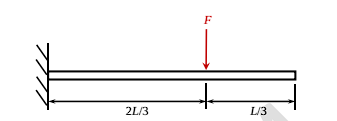
\includegraphics[width=0.5\columnwidth]{fig5.png}
\caption{}
\end{figure}

\begin{enumerate}
\begin{multicols}{2}
\item 1-2-3-6
\item 1-4-3-6
\item 1-5-6
\item 1-4-5-6
\end{multicols}
\end{enumerate}

\hfill (GATE PI 2025)

\item The benefit(s) of product standardization is/are

\begin{enumerate}
\item Need of less number of drawings
\item Reduction in unit cost
\item Reduction in inventory cost
\item Greater product variety
\end{enumerate}

\hfill (GATE PI 2025)

\item The value of the integral $\displaystyle \int_{1}^{3} \brak{x^{2}-2x}\,dx$ obtained by using Simpson's 1/3 rule with $4$ subintervals is equal to $\frac{n}{3}$. The value of $n$ is \dots. (Answer in integer)

\hfill (GATE PI 2025)

\item If $\mathbf{i}$, $\mathbf{j}$ and $\mathbf{k}$ are the orthogonal unit vectors in Cartesian $x$-$y$-$z$ coordinate system, the rate of change of the function $f\brak{x,y,z}=x^{2}+2y^{2}+z$ at point $\brak{1,\,1,\,1}$ in the direction of $3\mathbf{i}+4\mathbf{k}$ is \dots. (Answer in integer)

\hfill (GATE PI 2025)

\item In a wire drawing of a perfectly-plastic material with flow stress of 300 MPa, the back tension is zero and front tension is 200 MPa. Assuming ideal deformation with zero friction, the percentage reduction of the cross-sectional area of the wire is \dots. (Rounded off to one decimal place)

\hfill (GATE PI 2025)

\item In a cold rolling process without front and back tensions, the required minimum coefficient of friction is 0.04. Assume large rolls. If the draft is doubled and roll diameters are halved, then the required minimum coefficient of friction is \dots. (Rounded off to two decimal places)

\hfill (GATE PI 2025)

\item In a direct current arc welding, the voltage $V$ (in volt) is related to the arc length $l$ (in cm) as
\begin{align*}
V=\brak{30+30l}.
\end{align*}
The open circuit voltage is $80$ volts. The maximum possible arc length (in cm) is \dots. (Rounded off to two decimal places)

\hfill (GATE PI 2025)

\item A worker is allowed half an hour personal time in a normal 8-hour shift. If the normal time for manufacturing a product is $5$ minutes, the standard time (in second) is \dots. (Answer in integer)

\hfill (GATE PI 2025)

\item A product has to be manufactured in a single-line layout by carrying out the six tasks in a sequence. The time (in minute) of the six sequential tasks are 37, 8, 19, 34, 36 and 17. These tasks cannot be further sub-divided. For minimizing the cycle time, the number of stations to be used is \dots. (Answer in integer)

\hfill (GATE PI 2025)

\item A through hole of 1 mm diameter is to be drilled in a mild steel plate of 30 mm thickness. The selected spindle speed and feed for drilling hole are 600 revolutions per minute (RPM) and 0.3 mm/rev, respectively. Take initial approach and breakthrough distances as 3 mm each. The total time (in minute) for drilling one hole is \dots. (Rounded off to two decimal places)

\hfill (GATE PI 2025)

\item In the iron-carbon equilibrium phase diagram, the eutectoid reaction occurs at $723\,^\circ\mathrm{C}$ with the eutectoid composition of $0.83$ weight \% carbon. Ferrite and cementite phases are considered to contain 0.022 weight\% carbon and 6.67 weight \% carbon, respectively. If a steel specimen with $0.7$ weight \% carbon is cooled from $950\,^\circ\mathrm{C}$ to below $723\,^\circ\mathrm{C}$, the fraction of eutectoid ferrite is \dots. (Rounded off to two decimal places)

\hfill (GATE PI 2025)

\item During orthogonal cutting with a tool of $10^\circ$ rake angle, the cutting and thrust forces are $900$ N and $275$ N, respectively. The coefficient of friction on the rake surface of the tool is \dots. (Rounded off to two decimal places)

\hfill (GATE PI 2025)

\item In casting a cube of $80$ mm side, the volumetric shrinkages due to solidification and solid contraction are $4.5\%$ and $2\%$, respectively. Assume uniform cooling in all directions. The side (in mm) of the cubical pattern for getting the required size casting is \dots. (Rounded off to two decimal places)

\hfill (GATE PI 2025)

\item The solidification of a casting starts at 10 AM. However, the solidification of the molten metal at the center-line of the mold starts at 10:03 AM and ends at 10:10 AM. The casting is considered solidified completely when the solidification is completed at the center-line of the mold. The center-line feeding resistance (CFR) in percentage is \dots. (Answer in integer)

\hfill (GATE PI 2025)

\item A link $OA$ of length $200$ mm is rotating counter clockwise about $O$ in $x$-$y$ plane with a constant angular velocity of $100$ rad/s, as shown in the figure. The absolute value of the $x$-component of the linear velocity (in m/s) of point $A$ at the instant shown in the figure is \dots. (Rounded off to one decimal place)

\begin{figure}[H]
\centering
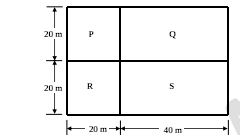
\includegraphics[width=0.5\columnwidth]{fig6.png}
\caption{}
\end{figure}


\hfill (GATE PI 2025)

\item A force of $1000$ N is acting at point $A$ on a bracket fixed at point $B$ as shown in the figure. The magnitude of the moment of the force about $B$ (in N.m) is \dots. (Rounded off to one decimal place)

\begin{figure}[H]
\centering
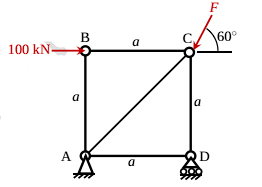
\includegraphics[width=0.3\columnwidth]{fig7.png}
\caption{}
\end{figure}


\hfill (GATE PI 2025)


\item A steel plate is fastened to a channel using three identical bolts as shown in the figure. The bolts are made of carbon steel of permissible yield strength in shear as $400$ N/mm$^{2}$. The plate is subjected to a force of $12$ kN. Neglect the weight of the plate. The magnitude of the resultant shear force (in N) on bolt 2 is \dots. (Answer in integer)

\begin{figure}[H]
\centering
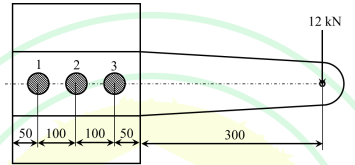
\includegraphics[width=0.5\columnwidth]{fig8.png}
\caption{}
\end{figure}


\hfill (GATE PI 2025)

\item The annual profit of a company depends on its annual marketing expenditure. The information of preceding 3 years' annual profit and marketing expenditure is given in the table. Based on linear regression, the estimated profit (in units) of the 4th year at a marketing expenditure of $5$ units is \dots. (Rounded off to two decimal places)


\begin{table}[htbp]
  \centering
  \caption{Table-7}
  \label{tab:tables/table7.tex}
  \begin{tabular}{cc}
  \textbf{Group-I} & \textbf{Group-II} \\ \\
    P. Chymosin & 1. Removal of cooked flavor from milk \\
    Q. Sulfhydryl oxidase & 2. Soyabean milk coagulation \\
    R. $\beta$-Galactosidase & 3. For rennet puddings \\
    S. Microbial proteases & 4. Lactose removal \\
  \end{tabular}
\end{table}
\hfill (GATE PI 2025)

\item Three plants $P_{1}$, $P_{2}$ and $P_{3}$ produce $6$, $1$ and $9$ thousand liters of fruit juice, respectively. The produced fruit juice is transported to three distribution centers $D_{1}$, $D_{2}$ and $D_{3}$ with requirement of $7$, $5$ and $4$ thousand liters of juice, respectively. The transportation cost (in hundreds of Rupees) from each plant to each distribution center is given in the table. The total transportation cost (in hundreds of Rupees) in initial basic feasible solution using Vogel's approximation method is \dots. (Answer in integer)

\begin{center}
\begin{tabular}{|c|c|c|c|c|c|}
\hline
Job & A & B & C & D & E \\
\hline
Processing time (in days) & 9 & 6 & 4 & 5 & 8 \\
\hline
\end{tabular}
\end{center}


\hfill (GATE PI 2025)

\item A company purchases items in bulk for getting quantity discount in the item's price. The price break-up is given in the table. The annual demand for the item is $5000$ units. The ordering cost is Rupees $400$ per order. The annual inventory carrying cost is $30$ percent of the purchase price per unit. The optimal order size (in units) is \dots. (Answer in integer)

\begin{table}[htbp]
  \centering
  \caption{Table-9}
  \label{tab:tables/table9.tex}
  \begin{tabular}{cc}
  \textbf{Group-I} & \textbf{Group-II} \\ \\
    P. Degumming & 1. Crystallization of triacylglycerol by cooling to remove fat crystals \\
    Q. Deacidifying & 2. Passing heated oil over charcoal \\
    R. Bleaching & 3. Using alkaline solution to remove fatty acids \\
    S. Winterizing & 4. Wetting with water to remove lecithin \\
  \end{tabular}
\end{table}

\hfill (GATE PI 2025)

 \item The zero line of the Vernier scale lies between divisions 20 and 21 of the main scale. The 4$^{\text{th}}$ Vernier scale division exactly coincides with a main scale division. The 5 divisions of the Vernier scale are equal to 4 divisions of the main scale. If one main scale division is 1 mm, the measured value (in mm) is \dots. (Rounded off to one decimal place)

\hfill (GATE PI 2025)

\item A broaching machine makes key slots with a mean dimension of $10.56$ mm and a standard deviation of $0.05$ mm. The upper control limit for mean of sample size $5$ calculated using X-bar $\brak{\bar{X}}$ chart is \dots. (Rounded off to two decimal places)

\hfill (GATE PI 2025)

\item The table shows the data of running a machine for five years. The original machine cost is Rupees $70,000$. In order to minimize the average total cost per year for running the machine, the machine should be replaced after \dots\ years. (Answer in integer)

\begin{table}[htbp]
  \centering
  \caption{Table-10}
  \label{tab:tables/table10.tex}
  \begin{tabular}{cc}
\textbf{Column-I} & \textbf{Column-II}\\

P. Aspergillus & 1. Arthrospore \\
Q. Geotrichum & 2. Oospores \\
R. Rhizopus & 3. Conidia \\
S. Oomycetes & 4. Sporangiospores \\
  
  
  
  \end{tabular}
\end{table}

\hfill (GATE PI 2025)


\item Water flows through a smooth circular pipe of diameter $10$ cm and length $10$ m. The pressure drop across the length of the pipe is $0.2$ Pa. Kinematic viscosity and density of water are $1\times10^{-6}$ m$^{2}$/s and $1000$ kg/m$^{3}$, respectively. Assuming laminar and fully developed flow throughout the pipe, the velocity of water (in mm/s) at the center of the pipe is \dots. (Rounded off to one decimal place)

\hfill (GATE PI 2025)

\item The left-hand side of a $20$ cm thick wall is maintained at $25\,^\circ$C. The right-hand side of the wall is exposed to hot air at $50\,^\circ$C. There is no heat generation inside the wall and its thermal conductivity is $100$ W/m.K. The convective heat transfer coefficient is $50$ W/m$^{2}.$K. Under steady state condition, the temperature (in $^\circ$C) of the right-hand side surface of the wall is \dots. (Rounded off to one decimal place)

\hfill (GATE PI 2025)

\end{enumerate}

\end{document}